%!TEX root = ../main.tex
%-------------------------------------------------------------------------------
\section{Example}\label{Example}
%-------------------------------------------------------------------------------
Our research group is actively developing the the \verb+respy+ package which allows for the flexible specification, simulation, and estimation of the typical EKW models. Details are available in its online documentation at \url{https://respy.readthedocs.io}. We now provide the seminal implementation of \citet{Keane.1994} as an example.

\paragraph{Setup} Individuals live for a total of $T$ periods and make a decision about their human capital investment each period. They choose to either work in one of two occupations (a = 1, 2), attend school (a = 3), or stay at home (a = 4). The immediate utility from each alternative is the following:
%
\begin{align*}
u_t(s, a) = \begin{cases} w_{1t} =
\exp\{\alpha_{10} + \alpha_{11}g_t + \alpha_{12}x_{1t} + \alpha_{13}x^2_{1t} + \alpha_{14}x_{2t} + \alpha_{15}x^2_{2t} + \epsilon_{1t}\} & \text{if}\; a = 1 \\
w_{2t} = \exp\{\alpha_{20} + \alpha_{21}g_t + \alpha_{22}x_{1t} + \alpha_{23}x^2_{1t} + \alpha_{24}x_{2t} + \alpha_{25}x^2_{2t} + \epsilon_{2t}\}& \text{if}\; a = 2 \\
\beta_0 - \beta_1 \Ind[\,g_t \geq 12\,] - \beta_2(1 - \Ind[\,a_{t - 1} = 3\,]) + \epsilon_{3t}& \text{if}\; a = 3 \\
\gamma_0 + \epsilon_{4t}& \text{if}\; a = 4. \\
\end{cases}
\end{align*}
%
$g_t$ is the number of periods of schooling obtained by the beginning of period $t$, $x_{1t}$ and $x_{2t}$ are the number of periods that the individual worked in the two occupations respectively. The utility for each labor market alternative corresponds to its wage $(w_{1t}, w_{2t})$ and $\alpha_{1}$ and $\alpha_{2}$ are thus parameters associated with the wage functions. They capture the returns to schooling and occupation-specific human capital. $\beta_0$ is the consumption utility of schooling, $\beta_1$ is the post-secondary cost of schooling, and $\beta_2$ is an adjustment cost associated with returning to school. The mean utility of the home alternative is denoted $\gamma_0$. The $\epsilon_{at}$'s are alternative-specific shocks to occupational productivity, the consumption utility of schooling, and the utility of home time. They are serially uncorrelated.\\

\noindent Given the structure of the utility functions and the lack of serial correlation, the state at time $t$ is:
%
\begin{align*}
s_t = \{g_t,x_{1t},x_{2t},a_{t - 1},\epsilon_{1t},\epsilon_{2t},\epsilon_{3t},\epsilon_{4t}\}.
\end{align*}
%
The observable components of $s_t$ evolve according to the following rules:
%
\begin{align*}
    x_{1,t+1}  &= x_{1t} + \Ind[\,a_t = 1\,] \\
x_{2,t+1} &= x_{2t} + \Ind[\,a_t = 2\,] \\
g_{t+1}   &= g_{t\phantom{2}}    +  \Ind[\,a_t = 3\,].
\end{align*}
%
The transitions of all observable components of $s_t$ are deterministic. However, there is uncertainty about the realization of its unobservable components. All unobservable components are jointly normally distributed with mean zero and covariance matrix $\vec{\Sigma}$.
%
\begin{align*}
[\epsilon_{1t}, \epsilon_{2t}, \epsilon_{3t}, \epsilon_{4t}]^T \sim \mathcal{N}_0(\vec{0}, \vec{\Sigma})
\end{align*}
%
When entering the model, individuals have no labor market experience $(x_{11} = x_{21} = 0)$ but ten years of schooling $(g_1 = 10)$. The idea is that individuals are about age 16 when entering the model in the first period and start out identically, different choices over the life cycle are then simply the cumulative effects of different shocks.

\paragraph{Parameterization} \citet{Keane.1994} outline a life cycle model of human capital investment under risk, so we rely on their parameterization as a baseline but instill individuals with an additional fear of model misspecification. The returns to schooling differ considerably between the two occupations. Schooling increases wages by only 4\% in the first occupation compared to 8\% in the second. We will thus refer to the former as blue-collar and the latter as white-collar going forward. Starting wages are considerably lower in the white-collar sector but wages increase more rapidly with occupation-specific experience compared to blue-collar wages. Own-work experience is highly valuable in both occupations. However, while white-collar wages increase with blue-collar experience as well, the opposite is not true. There is a consumption value of schooling of \$5,000 but the total cost of pursuing post-secondary education is considerable and amounts to \$5,000. Once leaving school, individuals incur a nearly prohibitive cost of \$15,000 for re-enrolling. Individuals are forward-looking but the future is discounted by 5\%. The random shocks are not correlated across alternatives. Further details about the parameterization are available in Appendix \ref{Parameterization}.

\paragraph{Interface} Figure \ref{Workflow example} illustrates the typical workflow with the \verb+respy+ package. The model is specified in the parameters and options specification.

\begin{figure}[ht!]\centering
\caption{Workflow example}\label{Workflow example}
\lstset{language=python, morekeywords={as}, ndkeywords={=}, ndkeywordstyle=\color{blue}, keywordstyle=\color{red}, commentstyle=\color{darkgrey}, emph={get_example_model, get_crit_func, get_simulate_func}, emphstyle=\color{violet}, basicstyle=\footnotesize, frame=lines}
\begin{lstlisting}
import respy as rp

params, options, _ = rp.get_example_model("kw_94_one")
simulate = rp.get_simulate_func(params, options)
df = simulate(params)

\end{lstlisting}
\end{figure}

\paragraph{Descriptives} We simulate the life cycle histories of 1,000 individuals for 40 periods. Figure \ref{Descriptives} shows the share of individuals choosing each of the four alternatives by period. Initially, roughly 52\% of individuals are enrolled in school but this share declines rapidly and only 19\% attain any post-secondary education. Right away, about 35\% of individuals are working in the blue-collar occupation.  Blue-collar employment initially increases even further to peak at 67\% as individuals are leaving school and entering the labor market. White-collar employment rises constantly over the life cycle but never reaches more than 35\%. About 5\% of individuals stay at home each period.

\begin{figure}[ht!]\centering
\caption{Choice patterns}\label{Descriptives}
\scalebox{0.35}{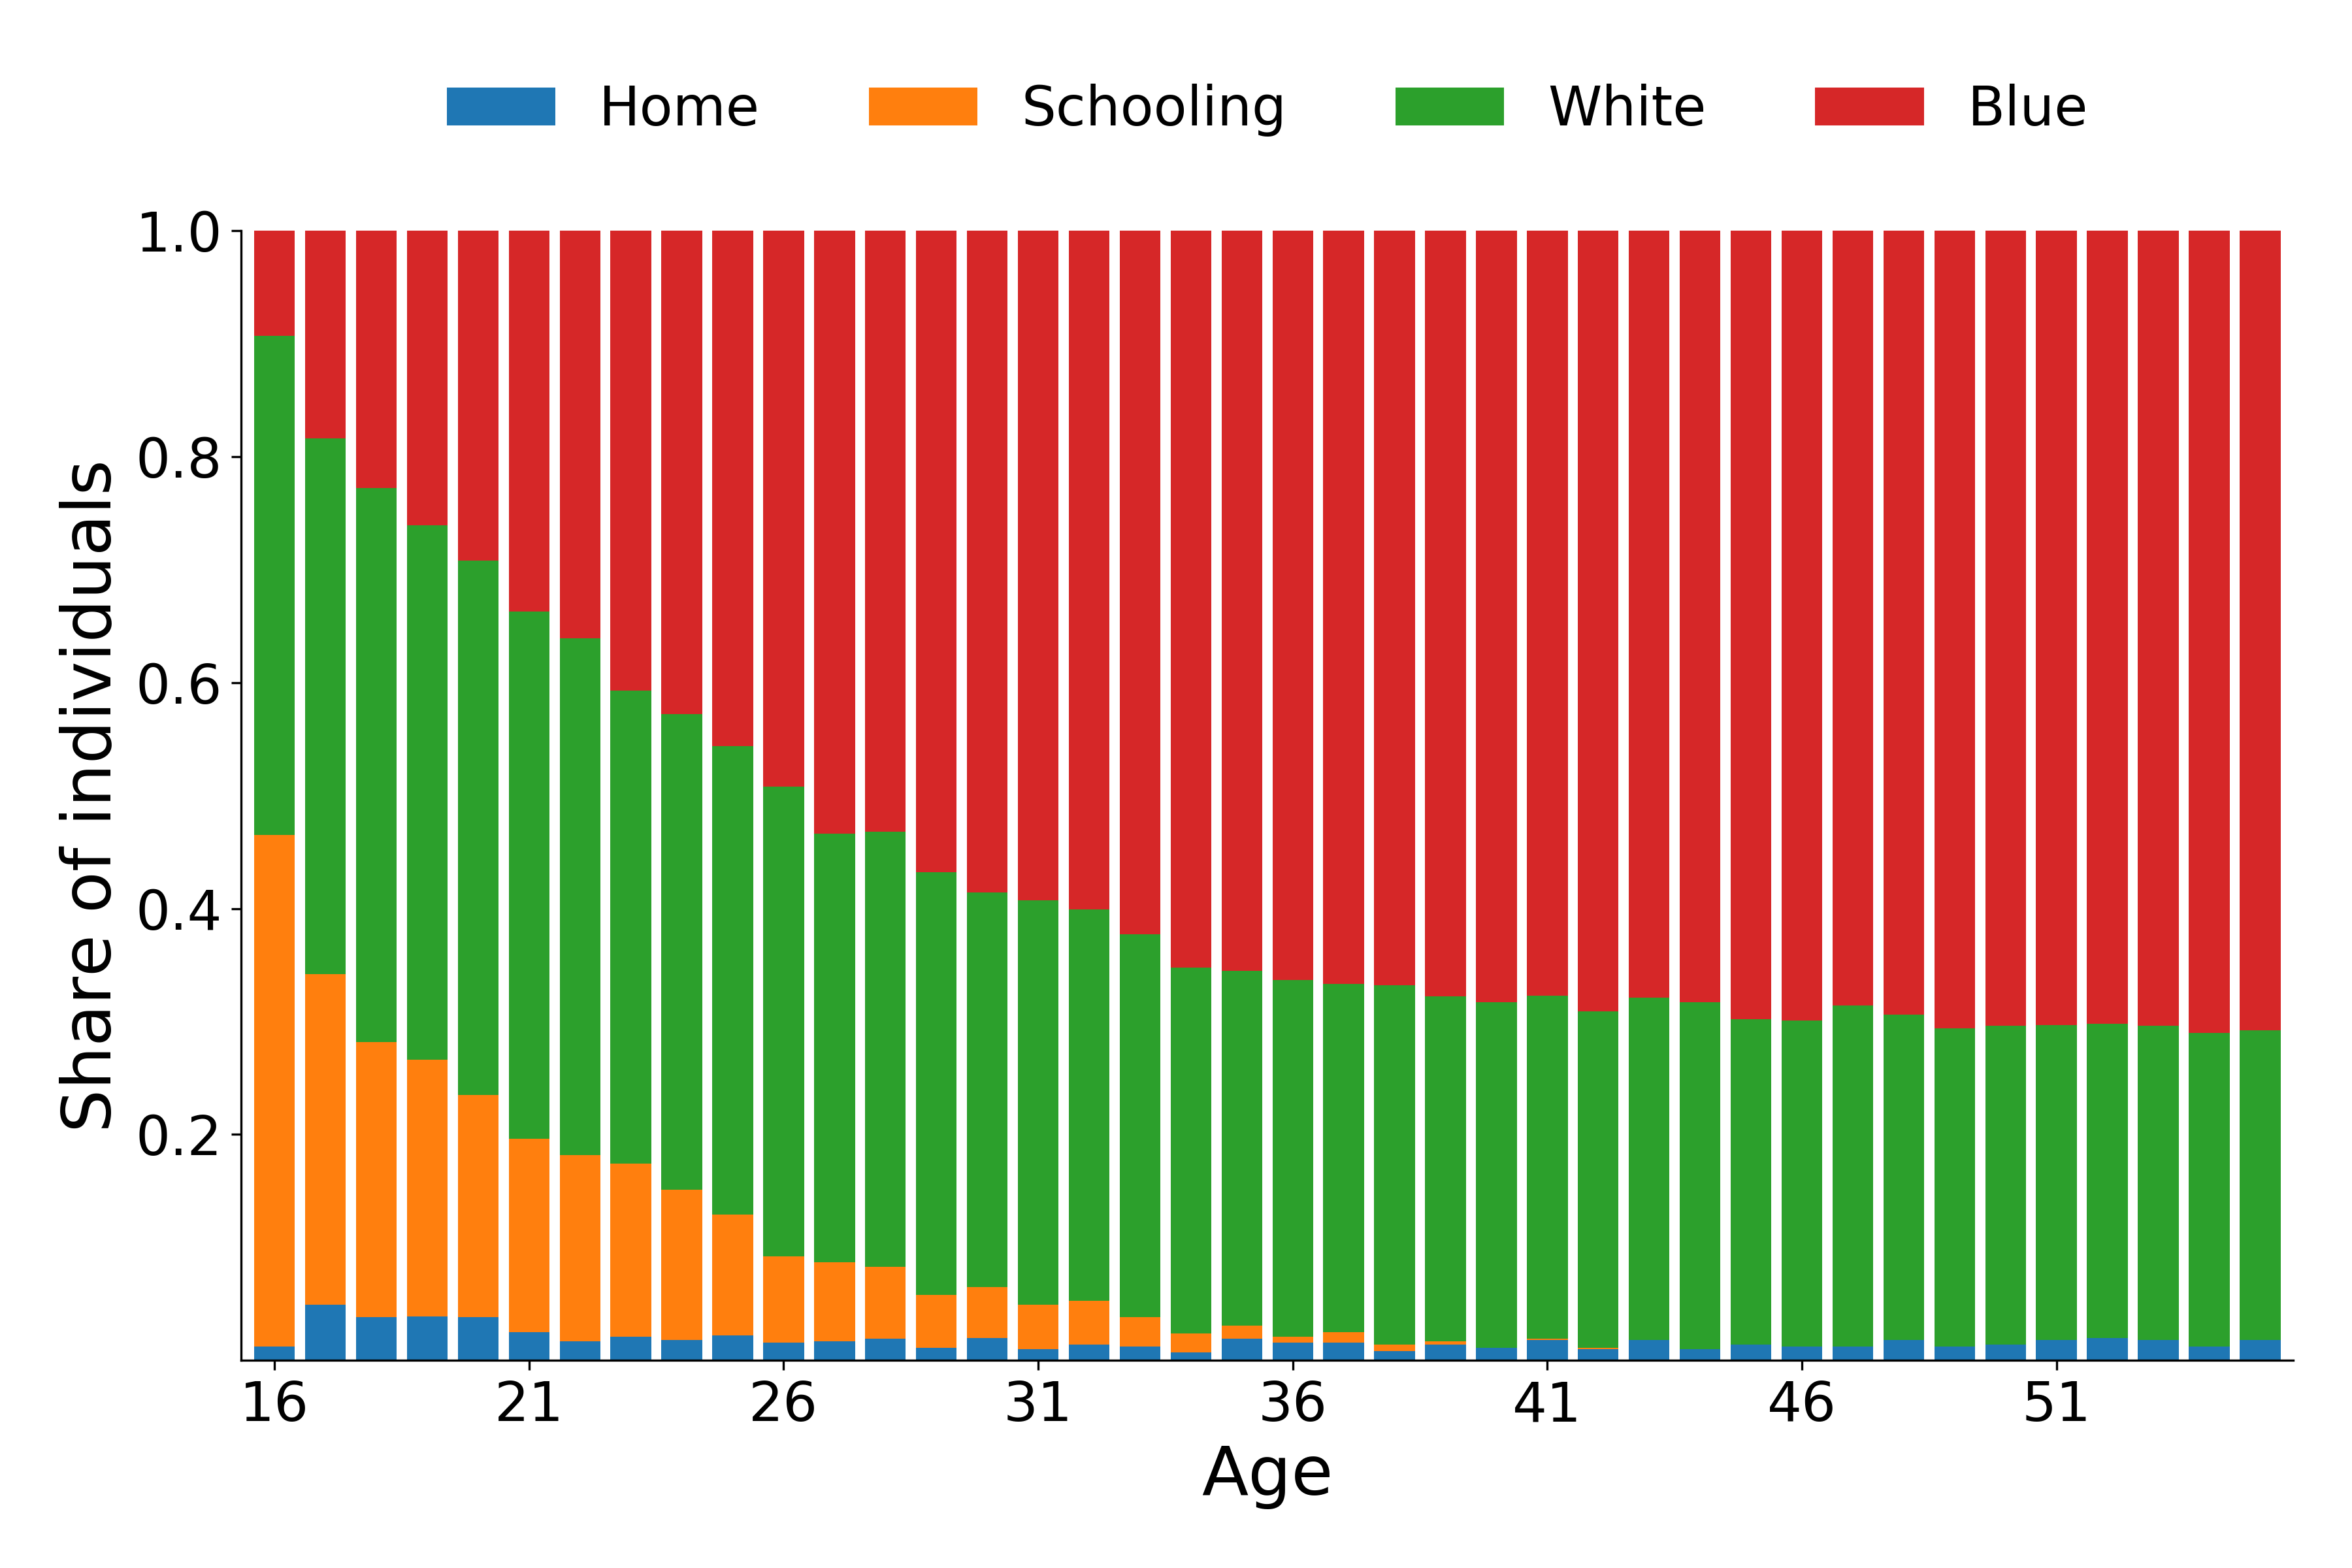
\includegraphics{fig-observed-choices}}
\end{figure}\FloatBarrier

\paragraph{Economic mechanisms and policy evaluation} Figure \ref{Economic mechanisms and policy evaluation} illustrates the ability of structural economic models to quantify the impact of economic mechanisms on average schooling and predict the effect of a tuition subsidy.  We evaluate the effect of a tuition subsidy of up to \$1.500 where we simulate a sample of 1,000 individuals but decrease $\hat{\beta}_1$ according to the tuition subsidy.

\begin{figure}[h!]\centering
\caption{Economic mechanisms and policy evaluation}\label{Economic mechanisms and policy evaluation}
\subfloat[Time preferences]{\scalebox{0.25}{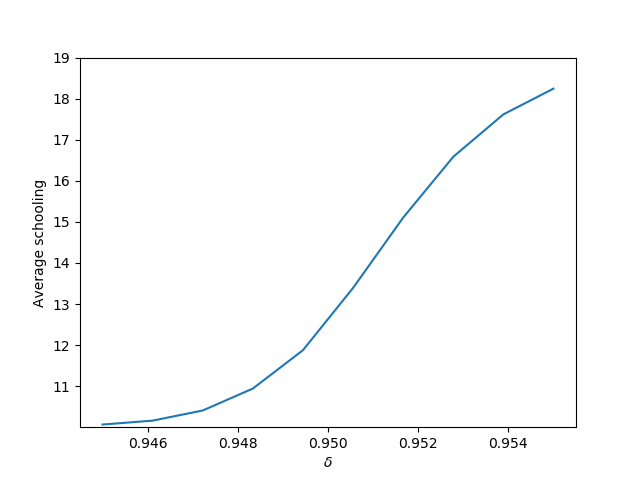
\includegraphics{fig-economic-mechanisms}}}\hspace{0.3cm}
\subfloat[Tuition subsidy]{\scalebox{0.25}{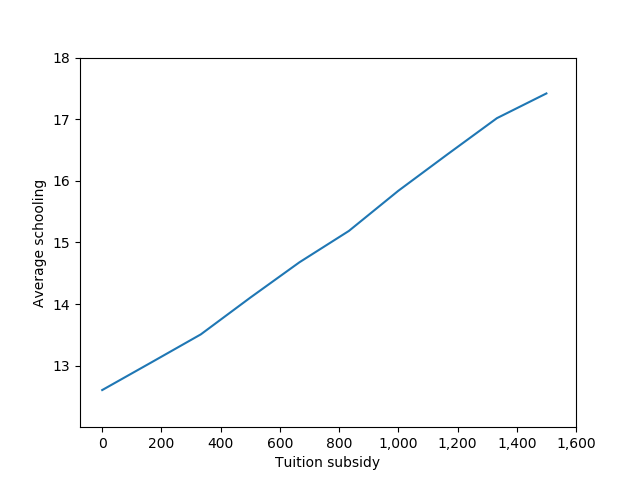
\includegraphics{fig-policy-evaluation}}}
\end{figure}
